\documentclass{article}

\usepackage[utf8]{inputenc}
\usepackage{graphicx}
\usepackage[margin=1in]{geometry}
\usepackage[numbers,sort]{natbib}
\usepackage{hyperref}

\hypersetup{
    colorlinks=true,
    linkcolor=black,
    urlcolor=blue,
    citecolor=black
}

\title{The Ecology of Cloud Computing}
\author{Alex H. Room}

\begin{document}
\maketitle



\section{Introduction}

In regards to the climate emergency, 'the cloud' is a rather apt metaphor for network computing; we are yet to learn whether it will provide us shade from a burning issue, or stand as an omen for a terrible storm. It has the potential to reduce the climate impact of several industries, but if not managed carefully it could cause our global emissions to skyrocket. This report will survey the current climate impact of scientific computing with case studies in particular pertinent areas and parts of scientific computing workflows, taking a particular focus on cloud computing and how we can take a variety of approaches to mitigate the extra overhead introduced by cloud facilities, finishing with a discussion on some present and future ideas on how to reduce our climate impact. \newline

This is a topic I have chosen due to my interest in sustainability, and noting that there is thus far very little research and discussion into the impact of computing on the environment; it is often seen as something which just happens on the screen and has no real existence outside the machine's case. Leading the current research into the field is Lo{\"\i}c Lannelongue, from whose work much of my understanding and research into the topic germinated; his contribution to a digestible and layman-friendly yet uncompromising introduction to the field is invaluable.

\begin{figure}[!ht]
\begin{center}
    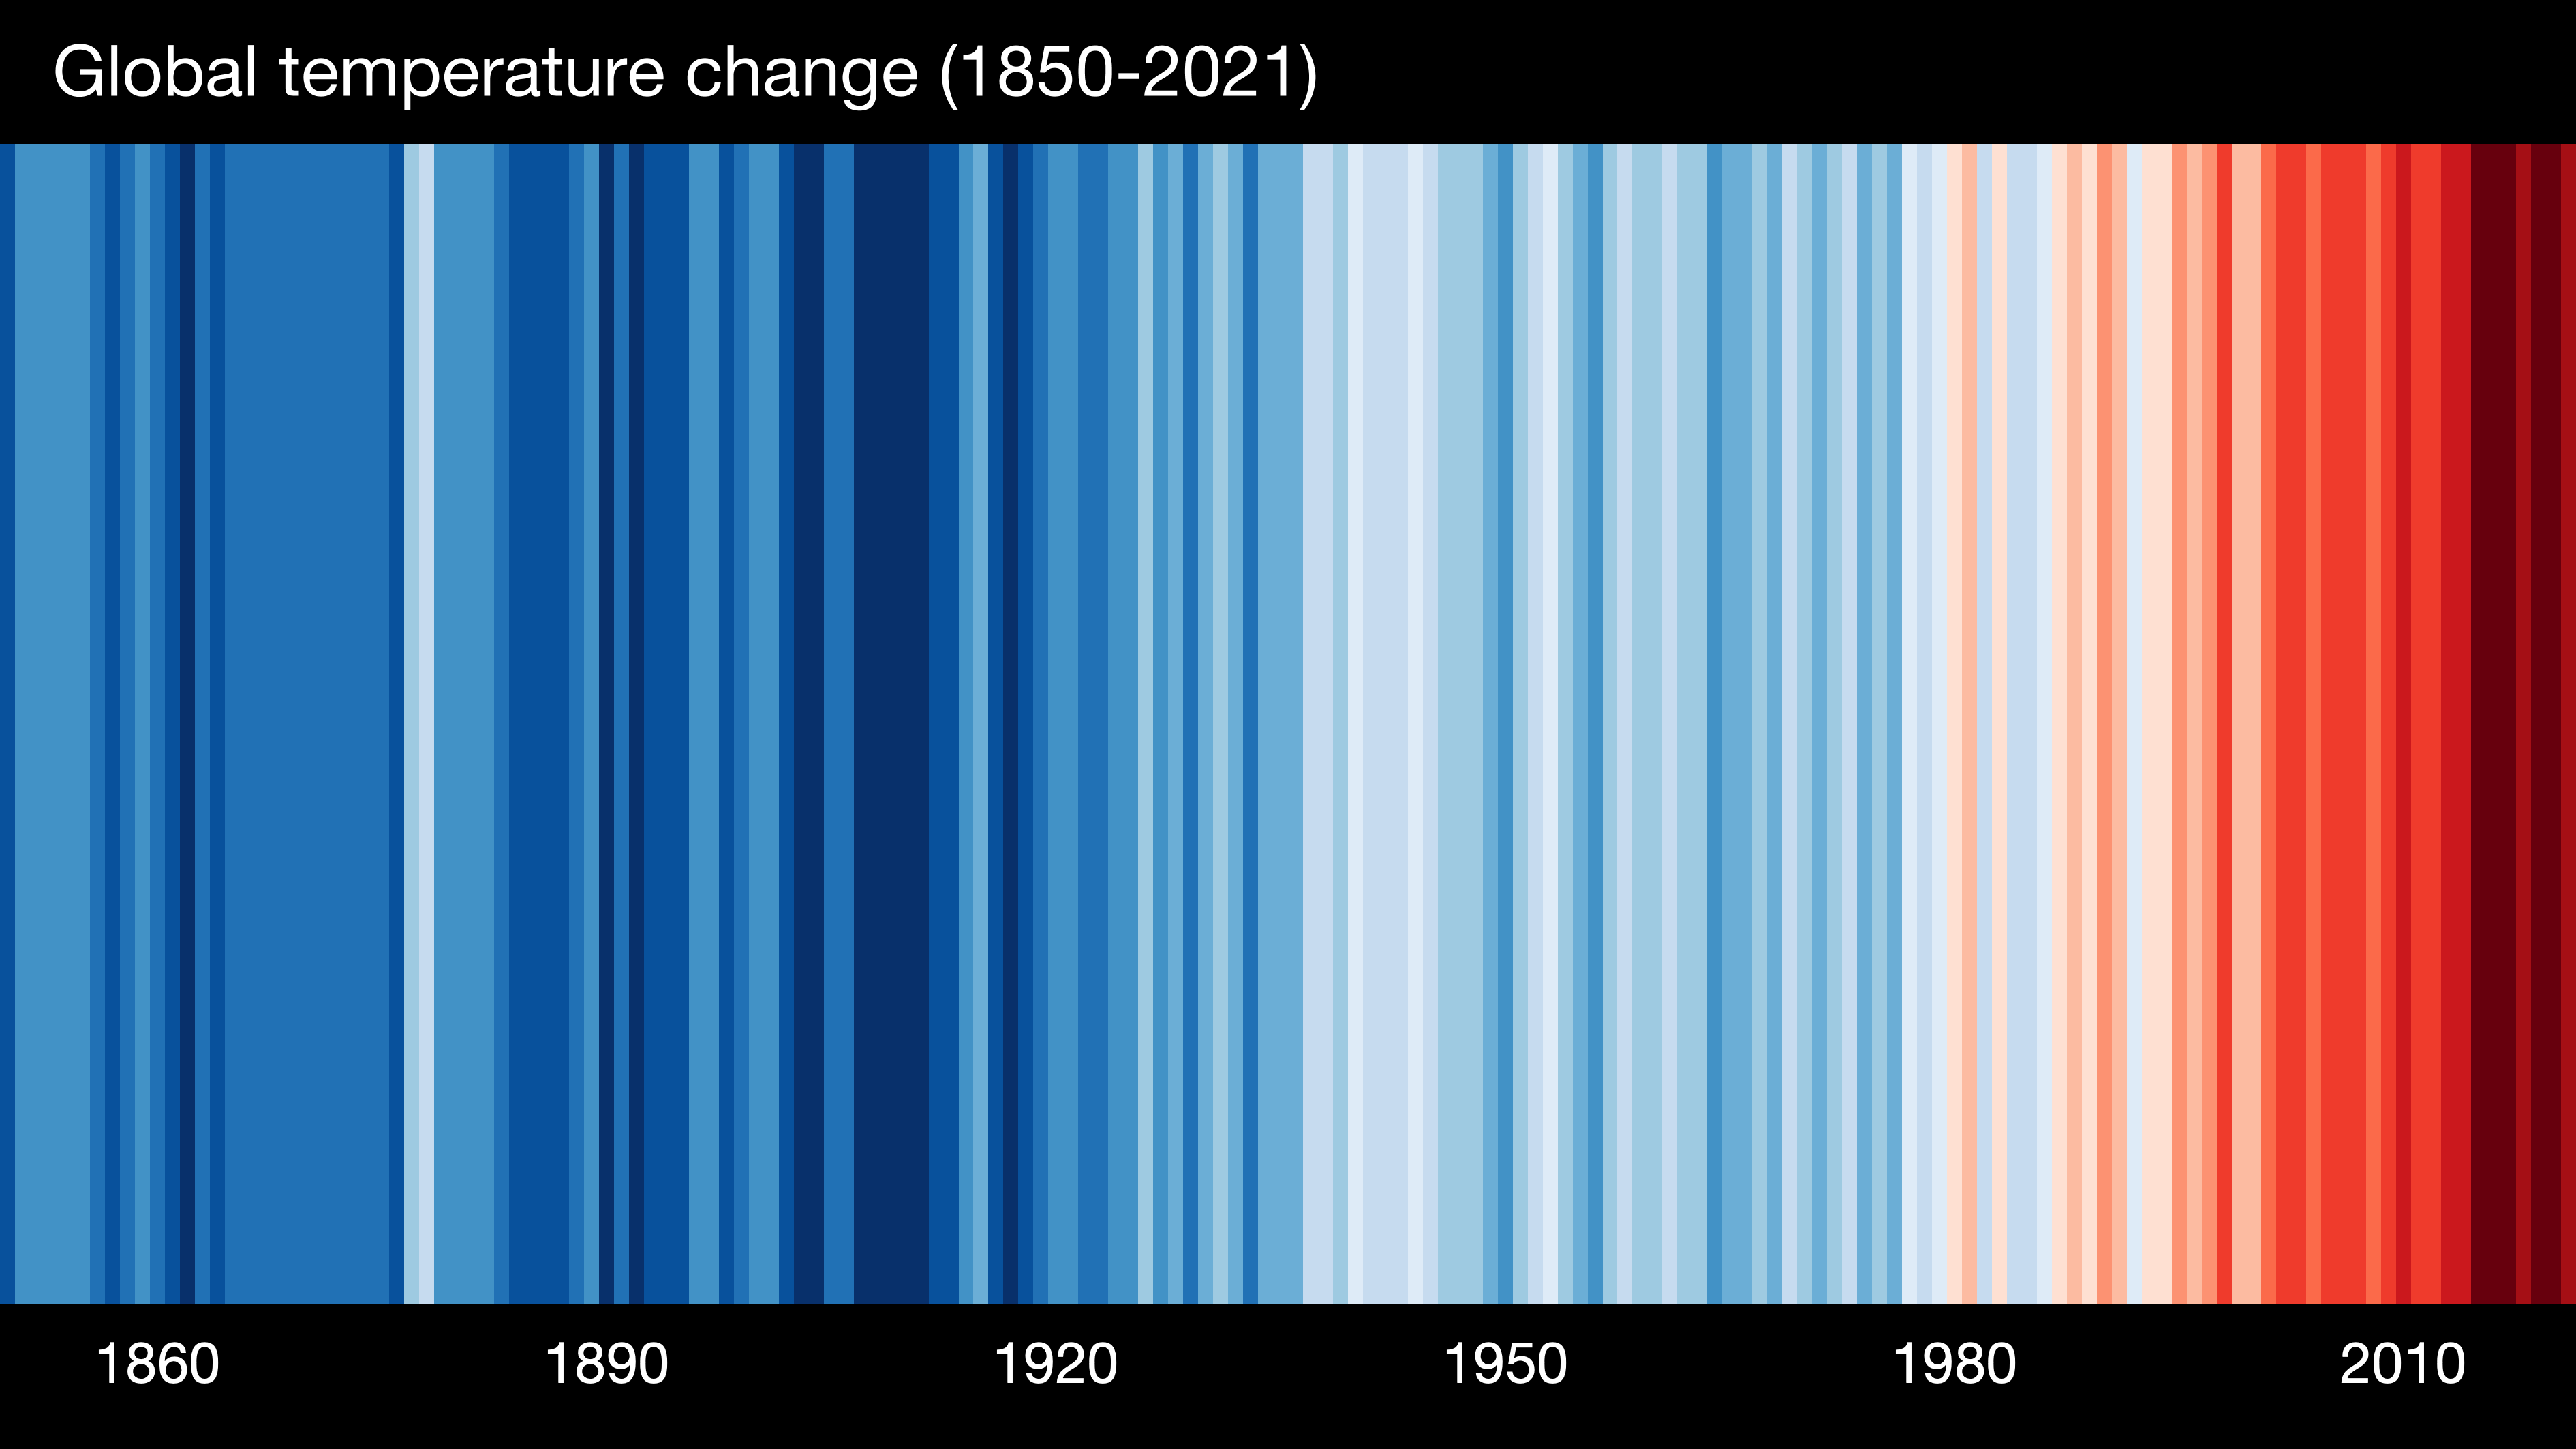
\includegraphics[width=.6\textwidth]{Diagrams/GLOBE---1850-2021-MO-withlabels.png}
        \caption{A graphic of global average temperature per year from 1850 to 2021 (I believe this image should be somewhere in every paper on anthropogenic climate change). \citep{hawkins2021show}}
\end{center}
\end{figure}

\subsection{What is cloud computing?}
Cloud computing is simply the ability to use computing resources (like storage or processing space) without having to directly own or manage them. For example, if we wanted to have our own website, we could buy a rack of servers ourselves, plug them into the wall, set them up, and voila: we have a website. But what happens when our website gets popular? What happens if one million people all want to use it at one time? We could keep scaling up, fill our kitchen with server racks, start buying air-conditioning for them, and deal with the rather large electricity bill - an approach that many now-huge websites once had to contend with, but eventually you run out of space and time to look after it all without significant investment. \newline

On the other hand, we could host our website on the cloud by renting servers in a data center somewhere. For example, Amazon's Elastic Compute Cloud (EC2) charges \$0.10 per hour for each computer you require, and only for the hours where the computers are actively running. You can host your website off their datacenter, and Amazon has dedicated people who look after the servers and make sure they are running correctly. As you can see, this is a very attractive alternative to self-hosting, particularly at large scales. However, when you do this, it is easy to forget about the real, physical equipment behind whatever computing you are doing - without care, we can fall into seeing the cloud as an abstract \emph{thing} that processes our data for us, an amorphous blob of circuits beyond concrete concerns. Without mindfulness, the emissions problem can thus easily slip out of our hands. 


\subsection{Some intuition for carbon use}
Most estimates of emissions are in the units CO2e, or "Carbon dioxide equivalent". This is to provide a standardised unit for emissions from different gases - for example, the climate impact of 1kg of methane is the same as the impact of 25kg of CO2 \citep{forster2007changes}, so if a process emits 3kg of methane and 4kg of CO2 it has emissions of $(3*25)+4=79$kg CO2e. Still, we generally do not have good intuition when it comes to knowing what 1g CO2e actually \emph{means}. Here are some benchmarks (the first three taken from \citet{lannelongue2021ten}):
\begin{itemize}
\item In a European car, driving one kilometre emits about 175g CO2e.
\item Flying from Paris to London emits around 50kg CO2e.
\item Streaming video for one hour emits around 55g CO2e (although this is hard to keep track of; electricity use from data transmission has halved every 2 years on average \citep{aslan2018electricity}).
\item The entire life-cycle of an iPhone 11 used for 3 years is 72kg CO2e (79\% of which is from manufacturing). \citep{apple2019product}
\item One kWh of electricity from the UK grid emits 233g CO2e. \citep{uk2020greenhouse}
\end{itemize}


\subsection{A miniature case-study of what can go wrong: NFTs}
One recent case of computing and climate that has caught media attention is the non-fungible token (NFT). 'Fungibility' is the ability of an object to have an equivalent copy - for example, gold is fungible (every kilogram of gold is worth exactly the same as every other kilogram of gold) whereas, say, a piece of artwork is not (if I were to make a duplicate of Van Gogh's Starry Night, it would not be as valuable as the real painting). \newline

An NFT uses an algorithm to create non-fungible digital data - like a digital certificate of authenticity. It uses a technology called blockchain to make a digital receipt that cannot be copied or faked. A blockchain is essentially a list (of transactions) and a signature - the signature is a line of letters and numbers that encapsulates the contents of the list. If someone tampers with the list, or tries to improperly add something to it, the signature and list will not match and you will be able to tell it has been tampered with.\citep{narayanan2017bitcoin} This can be a good thing; artists have found use in it, being able to sell digital art as a limited-stock item (like traditional paintings are) directly, without having to go through a middleman (e.g. an auction house). In fact, in 2020,  artists earned \$1.8 million \citep{redman2020NFT} from selling their art as NFTs.\newline

Now, where's the catch? The problem is how this uses blockchain. The generation of this signature takes a lot of computation; it is estimated that one NFT transaction generates about 48kg of CO2 \citep{atken2020unreasonable}, 14 times the footprint of mailing a physical art print, and 74000 times the footprint of buying something via bank transfer. \citep{qiu2021what} In fact, if you had turned on a laptop the day the Roman Empire was founded, and used it from then until December 2020, that laptop would have produced less carbon emissions than NFTs did in 2020. \citep{atken2020unreasonable} \newline

Finally, all this is done for an algorithm that may not even be necessary; an alternate blockchain algorithm called proof-of-stake produces the exact same result with only 1\% of the computing power. \citep{saleh2021blockchain} This case study gives a stunning parable on how computing, what we use it for, and what algorithms we use can have a huge effect on the climate.



\section{Scientific computing and energy}
Scientific computing is, essentially, the process of turning electricity into data. To this end, it can be difficult to reduce the amount of electricity used, as this often involves generating less data. Nonetheless, we can review where current and potential problems lie, and where there is room for improvement; it may be useful to view from an efficiency standpoint, where our "science per unit energy" can be improved.


\subsection{Processing}
The website \href{www.green-algorithms.org}{www.green-algorithms.org} \citep{lannelongue2021green} is an online tool that lets you see the carbon impact of an algorithm. One may not be surprised to learn that the main independent variable here is runtime. When performing computation, a server's power draw is roughly 4 times what it is when the computer is idle \citep{lannelongue2021ten}. Efficiency, then, is key here; for example, the bioinformatics algorithm BOLT-LMM has a 73\% lower carbon footprint on version 2.3 than it did on version 1.  \citep{grealey2021carbon} \newline

With the ever-increasing processing power and memory of modern computers, it can be easy to not see efficiency as so mission-critical, especially for small algorithms - shaving one microsecond of runtime off a popular algorithm might not seem like much, but if that algorithm is used a trillion times (which is not so far-fetched, when you consider algorithms like Fast Fourier Transforms or signal processing tools) you save 11.6 days of processing time (and 7kg CO2e) total.  As your program gets faster, there is also tendency to increase its scope and process larger data. This can create a 'rebound' effect \citep{lannelongue2021ten} that ends up turning your efficiency improvements into larger energy use. In this regard, restraint should be exercised, alongside careful consideration of how much data you actually \emph{need} to do good science.\newline

One final point is to consider the programming language used when it comes to efficiency benefits. \citet{heer2018speed} compares the time taken for various programming languages to estimate $\pi$ via the Leibniz method. He finds that compiled\footnote{'Compiled' means a language where a \emph{compiler} takes your code and turns it into an executable file, which you then run; 'interpreted' means the program is run directly as it goes along, line-by-line by an \emph{interpreter}.} languages such as Go or C++ are the fastest, taking 6-9.5 seconds, whereas some popular interpreted languages such as R or Python3 take 181-243 seconds. Of course, this is not to say that all code should be written in C++ lest we kill the planet. Not everyone knows every programming language, and there are non-speed-related benefits that put one language ahead of the other (like Python's accessibility and large number of addon modules, or R being the \textit{de facto} standard for statistics in the life sciences). Merely, we should more heavily consider it when assessing what language to start a project in. Carbon cost may sway the balance when we think about how many saved processing hours are worth the extra development hours\footnote{In particular, code for an experiment that only runs once may not be worth the extra development time of a more difficult language, but code for a long-lasting piece of sotware may be.}. \newline


\subsection{Data}
Once we have processed our data, what do we do with it? Data storage counts for around 10\% of data center energy usage, for a total of 20TWh per year \citep{shehabi2016united} - nearly 40x the energy used by all personal computers in the UK in a year.  \citep{waters2019energy} Moreover, large amounts of energy is needed to produce all this storage media - the manufacture of a Dell PowerStore9000T hard drive (one of their largest available) produces approximately 2765kg CO2e. \citep{dell2021powerstore} A possible and quite successful solution used for data archival is to move unused data to magnetic tapes; with careful discernment of what data needs to be at one's fingertips versus on a library shelf. Using tape can reduce the space and utilities needed for storage sixfold. \citep{moore2007disk}. \newline

This is probably the area where it is easiest to 'de-abstract' our thinking. As humans, we are used to thinking in space, and most of us in our daily lives run into trouble with our phone, laptop or cloud service running out of space for us just as easily as we run out of space in a bookshelf or spare room. On a corporate scale, we may want to think about the actual usefulness of our archives, and 'declutter' as needed. Do we need to keep data from a 10-year-old study that has since far been superseded? Could we offload older data onto relevant parties (essentially, contacting researchers and saying 'we can give you your data if you like, but we aren't keeping it ourselves')? Maybe we could take a page from libraries and keep usage statistics, shedding datasets that have not been touched or asked for in years? Perhaps in our heads we may do well to separate 'just in case!' from 'just for when...', and assess whether we are archiving or simply hoarding.


\subsection{Machine learning}
Machine learning is becoming \textit{en vogue} in scientific computing; it is being used for everything from improving early stage drug discovery \citep{imrie2021generating} to solving systems of differential equations. \citep{bhattacharya2020model} In essence, machine learning consists of two stages. The first is a 'training' stage, where a large dataset is processed by an algorithm in a machine; the second is a 'application' stage where the machine then uses what it has learned to make estimations about new data. For example, if I were training a machine to read handwritten letters (see \citet{deng2012mnist}), the 'training' dataset would be a big set of handwritten letters along with what they represent (telling the machine 'these 50 handwritten digits are all the letter 'a' etc.), and the machine would use an algorithm to figure out similarities and differences between letters. The 'application' stage would then be giving it a handwritten letter it hasn't seen before and it figuring out what letter it is from the data it gathered during the 'training' stage. This means machine learning can do a lot of busywork that we previously had to employ humans to do, like picking out good candidates for new drugs or typing up handwritten letters; essentially, it could be seen as a way of 'automating intuition'. \newline

This learning stage can take a lot of computation - the MNIST database from \citet{deng2012mnist} has 60,000 training letters. The Enron corpus (\citet[see][]{klimt2004enron}), a dataset of emails used for English language machine learning, contains 700,000 emails; each of these needs an algorithm to be run on it individually. The total process can take days, and for advanced applications can use  huge amounts of electricity. \citet{strubell2019energy} found that training one model using Google's state-of-the-art BART machine learning framework takes 79 hours, in the process using 1507kWh\footnote{This calculation accounted for the cost of cooling and maintaining the data center during this time, not just the actual processing.} (approximately the energy used by a UK household in six months \citep{waters2019energy}) and 326kg CO2e (!). Smaller frameworks, like the T2T framework, used around 27kWh and 5kg CO2e (which is still a non-negligible amount). \newline

While machine learning has been an amazing development in several fields, it runs the risk of overuse; some software concepts can almost become fashionable, with not enough consideration put into them. Note that the statistics in the previous paragraph were for \emph{training} a model - that is, we generated over 5kg CO2e and \emph{have not even solved any problems yet}. Compared to a non-machine learning approach, it is entirely possible that this lump sum of carbon right at the start will put its footprint far ahead of a non-learning-based software for essentially its entire lifetime - care must be taken that machine learning is the right tool for the job.


\subsection{Computing as supplement}
Declaring the discussion finished where software ends would be myopic. So far we have only spoken about software, as if the scientific process is to magically generate data and push it through an algorithm. Most scientific computing is a two-step cycle, where one alternates between analysing data with software and creating data with laboratory instruments. We set up our experiment, collect data, analyse it, then either collect more data or go home and write a paper, as necessary. Through computing, we can add a third step to this cycle (which absorbs part of the 'creating data' step) - simulation. \newline

This could be supplemented with an example.\footnote{NB: \emph{just} an example. Various other practical concerns vastly complicate this in real life; this simply illustrates the interaction of scientific equipment and computing.} The instruments at STFC's ISIS facility consume around 1.1MW.\citep{findlay2021practical} There are 38 instruments, so we take a rough average of 20KW per instrument. The Intel Xeon X3430 server, which is the highest-power-drawing core listed on green-algorithms.org \citep{lannelongue2021green}, draws 23.8W per core when active; for high performance computing, one may want to use 8 or 16 cores - we will go with 16 and take 380W power draw for the whole server. As a further assumption (we are going for a bad case here), we will say this server is in a data centre, so add the overhead of the datacentre (per server), which will make it 532W. This gives us an approximately 1:38 ratio of instrument power use versus computing power use. Now, here we have a fascinating figure indeed; if we run an algorithm for less than 38 hours and as a result need one fewer hour of instrument use, we have saved energy (and thus carbon!). \newline

This statistic can be a useful tool to consider priorities in where this simulation step can be leveraged. For example, if a department is trying to decide which simulation tool to put funding into, one with a 1:40 ratio may be more attractive than one with a 1:5 ratio. Although, one disadvantage is that this statistic means nothing concrete on an objective level. For a molecular analysis experiment, 1:40 may be very attractive (as one could feasibly reap those time-saving benefits), whereas for a bioinformatics study the complexity of biological processes like protein interactions would make it a struggle to do a significant simulation in that time. \newline

It is important to remember that a lot of scientific equipment (such as the ISIS facility) will likely never be green until the entire national grid is green; they simply use too much power. We can try to reduce it where we can (via methods like this), but to disparage the electricity use of these facilities in general belies the huge environmental benefits created through the scientific studies they make possible; the research into things like superconductors \citep{shang2018time} or creating sustainable synthetic versions of natural resources that is only possible through huge facilities like this.



\section{Cloud computing}
Now we will specifically look at cloud computing; the benefits and drawbacks of moving our data to a dedicated external centre.


\subsection{Data centres}
A key factor in considering cloud computing is the idea of 'overhead' - around 40\% of the energy use of a datacenter is purely the energy used to cool it so the servers do not overheat,  \citep{lannelongue2021ten} which would not be necessary in a local server (which is small enough to be cooled effectively by similar techniques as those used to cool human beings). However, as datacentres are geared purely towards the processing and storage of data, this can be done more efficiently. In fact, a 2013 case study (\citet{masanet2013energy}) suggested that by moving common applications used in a company from a local server to the cloud, they could reduce emissions by 87\%\footnote{Not to mention the further reduction in emissions if employees are then able to work from home; if everything is on the cloud anyway, then why would they need to burn petrol to commute?}. Naturally, one large cloud centre can utilise efficiency 'economies of scale' better than dozens of local, small ones. Over time, this has certainly shown; research by Google found that while data centre use increased by 550\% between 2010 and 2018, the amount of energy consumed by datacentres only increased by 6\%, meaning the proportion of global energy used by datacentres did not increase despite their much greater usage. \citep{masanet2020recalibrating}\newline

If using a commercial data centre, one can find a better datacentre by shopping around for better carbon options; with the choice of any cloud provider in the world, you also have the choice of what country's grid they are plugged into. For example, generating one kWh in Switzerland emits 12g CO2e, while in Australia it is 880g. \citep{grealey2021carbon}. Another statistic of data centre efficiency is its PUE (Power Usage Effectiveness), which measures efficiency of a datacentre via the following ratio:

$$PUE = \frac{\textrm{Total facility energy use}}{\textrm{Server energy use}}.$$

Naturally, the ideal PUE is 1. The average datacentre has a PUE of around 1.67, but efficiency improvements can go much lower; for example, Google's datacentres have an average PUE of 1.1. \citep{holzle2020data}\newline

The PUE of a data centre can be reduced through various considerations; the first is how to manage heat emissions. Cooling the servers using water cooling rather than air conditioning (in fact, air conditioning has recently come under fire for creating a vicious cycle as the energy from air conditioning heats the planet, which means more air conditioning is required, and so on \citep{ospina2018cooling}) can be much more efficient. Design can be used to further improve this; a common way of cooling data centres is by cooling alternating rows of servers while letting the odd rows heat up, which creates a convection current around the whole room that keeps everything cool. The water cooling itself can also be made more effective using ground (passive) cooling - by piping the water underground before piping it back into the data centre, we can take advantage of the effectively unlimited cold under the earth. \newline

We can also integrate some interesting computing approaches to infrastructure to reduce PUE. \citet{evans2016deepmind} reduced the energy use for cooling at a Google datacentre by 40\% through training an AI on centre infrastructure data such as temperatures, power, pump speeds (for water cooling) and then allowing it to control the datacentre's cooling system. However, for 'smaller wins', we must consider the power use of our computing approaches; the actual energy use of training and running this AI may be non-negligible (although in this case, probably less than 40\% of the cooling bill). \newline

If building one's own datacentre, we can also save energy by using renewable energy sources. The main issue with this is in the case of methods like photovoltaic (solar) power, where their non-constant output could cause problems for a facility which needs to be on 24/7.\newline

Additionally, we can leverage the interplay of the datacentre areas vs the human areas; waste heat from servers can be used to heat up areas containing people rather than separate central heating. One incredibly simple way of doing this is to have areas designed for people on higher storeys, so the heat can rise and do as such. \newline

Finally, when processing data and running algorithms in our datacentre, better management and options for users can improve efficiency. One idea could be a 'queueing' system; if not in a rush to get results as soon as possible, users could be given the option to queue their processing for off-peak times where the system would otherwise be wasting electricity just idling away.


\subsection{Moving costs}
When we move our data over to a cloud centre, we must choose how we move it, as well as how we move large data back and forth from user to server in future. Thus, time for an interesting comparison; the carbon use of data transfer versus that of a heavy-goods vehicle. Huge corporations like Google transfer data using 'SneakerNet' - that is, loading hard drives into a van and taking them physically to their destination.\footnote{A wonderful article comparing SneakerNet to traditional bandwidth here: \href{https://what-if.xkcd.com/31/}{https://what-if.xkcd.com/31/}} As long as travel time is under 57 hours, SneakerNet is more efficient than the internet in terms of transfer speed \citep{jaya2020sneakernet} - for reference, crossing the United States takes 40-50 hours. But what about carbon? \newline

Data transmission emits a flat rate of CO2e per GB transferred, regardless of distance of transfer. A vehicle emits a certain amount of CO2e per kilometre. From this, we can create a simple equation for how much carbon Sneakernet emits compared to internet transfer (assuming that we are not transferring so much data that we cannot fit it all in one vehicle).

$$SC = E_{vehicle}d - E_{internet}s$$

where $SC$ is the relative Sneakernet carbon (how much carbon emitted by Sneakernet relative to that emitted by internet transfer), $E_{vehicle}$ is the emissions of the vehicle (in g CO2e/km), $d$ the distance of transfer (in km), $E_{internet}$ the emissions of data transmission (in g CO2e/GB) and $s$ the size of the data being transferred (in GB). A 2016 study estimated the energy cost of data transfer as 0.023kWh per gigabyte. \citep{aslan2018electricity} In the United Kingdom, this would emit 5g CO2e/GB. We will take our vehicle as a Mercedes Sprinter (the van used by Royal Mail), which emits approximately 192.6g CO2e/km. \citep{mercedes2019sprinter} We will say our facility is in central London, and our data centre at the Cyxtera Data Centre Campus, a popular data centre campus in Slough - a distance of around 35km. This creates a linear plot from which we can see Sneakernet's carbon emissions break even to the Internet's at a data size of 1348.2GB; that is just one or two regular-sized hard drives! This is even better with electric vehicles; Royal Mail plans to switch to the electric Arrival van, which at full capacity stores 139kWh with a range of 340km \citep{hubbard2021new}. If charged using fossil-fuel generated electricity (the worst-case scenario) this emits 94g CO2e/km, meaning we 'break even' on SneakerNet at 658GB, which one could probably fit on a single laptop. \newline

An even better-case scenario is if you are building your data centre on the same campus as your facility. Most data centres have a room known as a \emph{meet-me room}, or MMR, where people can enter and physically connect their personal device to the centre, letting them transfer data quickly in person. In this case, SneakerNet will almost certainly win out over data transfer, as the carbon output of walking across a campus is negligible. \newline


\subsection{A note on carbon offsets}
It is tempting to consider balancing out the extra electricity use of our datacentre with carbon offsetting. Carbon offsetting is the act of spending money on things with a negative carbon cost to counteract the emissions of a process. This ranges from practices like giving money to reforestation companies, to slightly more dubious things like investing in carbon sequestration research. \newline

Care must be taken when using carbon offsets. At best, they are an important part in a carbon-reduction portfolio, one which actually puts financial incentive on \emph{keeping} ecosystems rather than destroying them for profit. At worst, they are a way for an organisation to funnel money into reducing their climate guilt. It is important to deeply consider offsetting methods; for example, planting trees sounds like a brilliant idea (a mature tree sequesters 11kg of CO2 per year \citep{akbari2002shade}), but it takes 20 years before a tree is mature enough to start sequestering any significant amount of carbon \citep{ghussain2020biggest}. By this point, we may have long passed a point of no return for destructive climate change. Besides, are the partners we use for offsetting reliable? Are they protecting those trees? If your trees catch fire or are eaten by a deer as saplings, your offset may go entirely unrealised. \newline

A great case study where badly thought-through tree planting has been destructive for the Earth was the UK Government's 1981 Forestry Grant Scheme. To increase the UK's timber supply, the UK Government offered huge tax concessions to people who planted trees. \citep{watkins1983public} This concession was incredibly attractive to the super-rich, and soon people started looking for large tracts of land to plant these trees. Eyes moved to the Flow Country in the Scottish Highlands - a vast peatland, the largest bog in Europe. Roughly 500,000 hectares (5000 square kilometres) were drained and planted with conifers before the ecological importance of the Flow Country was recognised and the scheme ended; this was eventually done for the protection of habitats. 

The other importance of the Flow Country, unknown at the time, was the incredible carbon storage potential of the peatland; peatland bogs only make up 3\% of the world's land area, but store up to a \emph{quarter} of all the world's soil carbon. \citep{turetsky2015global} Worse still, when drained, they emit carbon rather than storing it; roughly 2 billion \emph{tonnes} of carbon dioxide are emitted from drained peatlands, making 5\% of all global human-created greenhouse gas emissions; not to mention that the trees planted on top of it grew poorly in the soil, and were essentially useless as timber. A badly-planned and badly-informed piece of environmental policy in the 1980s thus left huge ecological damage that Scotland is still working on repairing even today. \citep{gewin2020peat} \newline

One could make the analogy that carbon offsetting is the climate equivalent of the payday loan. Sure, your carbon output will balance out (over infinite time), but if you can help it it would be better to just leave the fossil fuels in the ground in the first place - and worse, a badly thought-out payday loan could put you in worse financial straits than you were in to start with.


\subsection{Futurism}
The future, like offsetting, is not to be relied on; we must think carefully about the environment now, rather than relying on scientists for a \emph{deus ex machina}. That said, there are some promising and interesting developments.\newline

The first is DNA data storage. This is where we artificially create DNA chains to store digital information. Not only is this method several orders of magnitude denser than magnetic tapes, it also can remain stable for hundreds or thousands of years, as well as a greener production life-cycle; its biological nature means it can biodegrade when no longer needed, rather than going to landfill or being incinerated. \citep{nguyen2020architecting}\newline

Another area of interest is quantum computing - this uses concepts from quantum physics to redo computing in a more efficient way 'from scratch'. Quantum computing involves the use of 'qubits', which take advantage of the uncertainty present in quantum-mechanical information to have more states than the 0 or 1 of a classical computing bit, and leverage this for incredibly fast computation. \citep{national2019quantum} The difference that this will make to the environment is completely unimaginable; it is estimated to be capable of quickly working through algorithms that normal computers could not do between now and the end of the universe, which completely changes the lens through which we see computing efficiency. \citep{gyongyosi2019survey} However, we cannot tell if the infrastructure required will balance it out in early days; as it stands, quantum computers must be supercooled to work, which uses a massive amount of cooling energy even on a very small scale. In fact, a sub-field of research into quantum computing is whether it is possible to make large quantum computers without the excessive heat causing the quantum components to fail. \citep{ikonen2017energy}\newline

One direct environmental application of quantum computing is its ability to solve complex problems in renewable energy. Controlling and balancing a far more decentralised national grid (i.e. one with thousands of distributed renewable energy sources, rather than a few dozen fossil fuel plants) is an incredibly complex problem that current supercomputers do not have the resources to solve; it is simply too many variables to keep track of to forecast future supply and demand like the grid currently does. Other energy problems include the modelling of battery designs; simulation (which is heavily based in keeping track of the positions and movements of thousands and thousands of molecules) is an area where quantum computing is likely to create huge speed impacts. \citep{giani2021quantum}

\section{Conclusion}
The main idea flowing through this report is one of care; one of mindfulness. There are countless ways to improve the efficiency of our computing and cloud facilities so long as one simply cares about them - the climate crisis is a modern, global elephant in the room and it should equally be an elephant in project planning. Somebody who does not care about the climate (at their own peril) could create scientific software, could hire servers in a datacentre, could perhaps even build their own datacentre, not considering these factors. But you, the reader, are more careful than that; we should be acutely aware of our electricity-based carbon emissions in the same way we are aware of the plastic we are putting in our general waste or fumes coming out of our cars. It shouldn't be an 'out of sight, out of mind' problem, but we know it is an inevitability that we will produce this waste as part of our lives.\newline

There is a default set of questions that we ask when we carry out a project. We ask 'is this going to be useful?', 'is this user-friendly?', or 'is my new building accessible to disabled people?'. Perhaps it is time to add a new question; "does my project work for the environment, or against it?" Can we at least work in harmony with environmental goals, or even better, contribute to them? You don't even have to care about the environment to do this - more eco-friendly businesses have better job satisfaction with less burnout and turnover \citep{yu2020hotels} \citep{reverte2016influence}, better perception from consumers \citep{miles1993eco}, and have an easier time recruiting new and better talent \citep{aranganathan2018green} - the latter two growing more and more important, as younger, more environmentally-conscious individuals begin to join the workforce (and consumer perception is, naturally, potential employee perception).\newline

Thus, it shouldn't be all or nothing; we should make a careful assessment of where we can reduce our energy use, and where we cannot. I try to evoke a future where we let the environment sway our judgements and play a factor in our science and scientific software. That way, it is possible to use the technology of the 'information age' in a way that is beneficial for both people and the planet.

\bibliographystyle{unsrtnat}
\bibliography{bibliography}
\end{document}